\chapter{Modelo de bolsa}
\label{ch-BagModel}

\pagestyle{fancy}
\fancyhf{}
\fancyhead[LE]{\nouppercase{\textbf{\leftmark}\hfill\textit{\rightmark}}}
\fancyhead[RO]{\nouppercase{\textit{\rightmark}\hfill\textbf{\leftmark}}}
\fancyfoot[LE]{\nouppercase{\thepage\hfill Pressure Distribution Inside Nucleons in a Tsallis-MIT Bag Model}}
\fancyfoot[RO]{\nouppercase{Pressure Distribution Inside Nucleons in a Tsallis-MIT Bag Model \hfill \thepage}}

\begin{chaptersummary}[Resumen del capítulo \thechapter: Modelo de bolsa]
    Este capítulo introduce el modelo de bolsa del \gls{mit} como marco fenomenológico para el confinamiento de quarks. Se parte de los fundamentos físicos provistos por la \gls{qcd} y se justifica el modelo desde la libertad asintótica, la inclusión de gluones y la estructura relativista-invariante. Se desarrolla formalmente la versión esférica del modelo, derivando sus ecuaciones de movimiento, condiciones de frontera y soluciones modales, que constituyen la base sobre la cual se construye la extensión no extensiva que proponemos más adelante.
\end{chaptersummary}
    
\section{Motivación y fundamentos desde la QCD}
    
Comprender cómo los quarks se confinan dentro de los hadrones ha sido uno de los desafíos más importantes de la física de partículas. Aunque la \gls{qcd} provee el marco teórico fundamental para describir las interacciones fuertes, su naturaleza no perturbativa a bajas energías hace difícil una solución exacta para sistemas ligados como los bariones. En este contexto, los modelos fenomenológicos como el modelo de bolsa del \gls{mit} ofrecen una herramienta útil para capturar aspectos esenciales de la dinámica hadrónica.
    
El modelo de bolsa parte de tres principios motivados por la \gls{qcd}:
    
\begin{enumerate}[a)]
\item \textbf{Confinamiento y libertad asintótica:} Los quarks están confinados a una región finita de espacio, pero se mueven libremente dentro de ella debido a la debilidad de las interacciones a corta distancia.
\item \textbf{Inclusión de gluones:} Aunque no siempre se introducen explícitamente, las correcciones debidas al intercambio de gluones son esenciales para describir propiedades del espectro hadrónico.
\item \textbf{Condición de singlete de color:} Solo estados globalmente neutros (singletes de color) son permitidos, lo cual es consistente con la ley de Gauss aplicada a campos de color confinados.
\end{enumerate}
    
A partir de estas ideas, se construye un modelo donde los quarks están confinados dentro de una “bolsa” esférica, cuyo tamaño y energía total resultan del equilibrio entre presión interna y presión de vacío externo, modelada por una constante \( B \) conocida como presión de bolsa.

\section{Formulación del modelo en cavidad esférica}

El enfoque formal del modelo parte de la acción para un campo de quarks sin masa en una cavidad esférica \cite{DeTar_1983}, dada por:

\begin{equation}
W = \int dt \left[ \int_{V} d^3x \left( \frac{i}{2} \bar{\psi} \overleftrightarrow{\partial}_{\mu} \gamma^{\mu} \psi - B \right) - \frac{1}{2} \int_{S} d^2x \bar{\psi} \psi \right]
\end{equation}

Este modelo asume:

\begin{enumerate}[i.]
\item Los quarks se comportan como partículas libres dentro de la cavidad.
\item Fuera de la cavidad, el vacío tiene menor energía, impidiendo la propagación de los campos.
\item Las condiciones de frontera imponen confinamiento y cuantizan las soluciones posibles.
\end{enumerate}

A partir de esta acción se derivan las ecuaciones de movimiento (la ecuación de Dirac) y condiciones de frontera que aseguran el confinamiento de quarks y el equilibrio de presiones. Las soluciones modales resultantes definen una base completa para construir estados hadrónicos dentro del modelo.

\section{Modelo de bolsa: descripción preliminar}

El modelo de bolsa del \gls{mit} ofrece una descripción fenomenológica del confinamiento de quarks, en la cual estos se encuentran libres en el interior de una región finita del espacio —la bolsa— y no pueden escapar debido a una presión negativa que actúa como barrera. En este esquema, los quarks se tratan como partículas relativistas sin masa dentro de la bolsa, mientras que el vacío exterior se modela como un medio con energía más baja.

Esta diferencia energética entre el interior y el exterior se modela mediante la llamada \emph{presión de bolsa} \( B \), que actúa como un parámetro fundamental para estabilizar el sistema. El tamaño de la bolsa queda entonces determinado por el equilibrio entre:

\begin{enumerate}
    \item[$\triangleright$] La \emph{energía cinética} asociada al confinamiento cuántico de los quarks,
    \item[$\triangleright$] y la \emph{energía volumétrica} proporcional a \( B \), que penaliza el crecimiento del volumen.
\end{enumerate}

Este modelo fue originalmente formulado por el grupo del MIT \cite{Chodos_1974} y ha sido extensamente utilizado para estimar propiedades de los hadrones ligeros, tales como sus masas, radios y momentos magnéticos.

\begin{wrapfigure}{l}{0.55\textwidth}
    \centering
    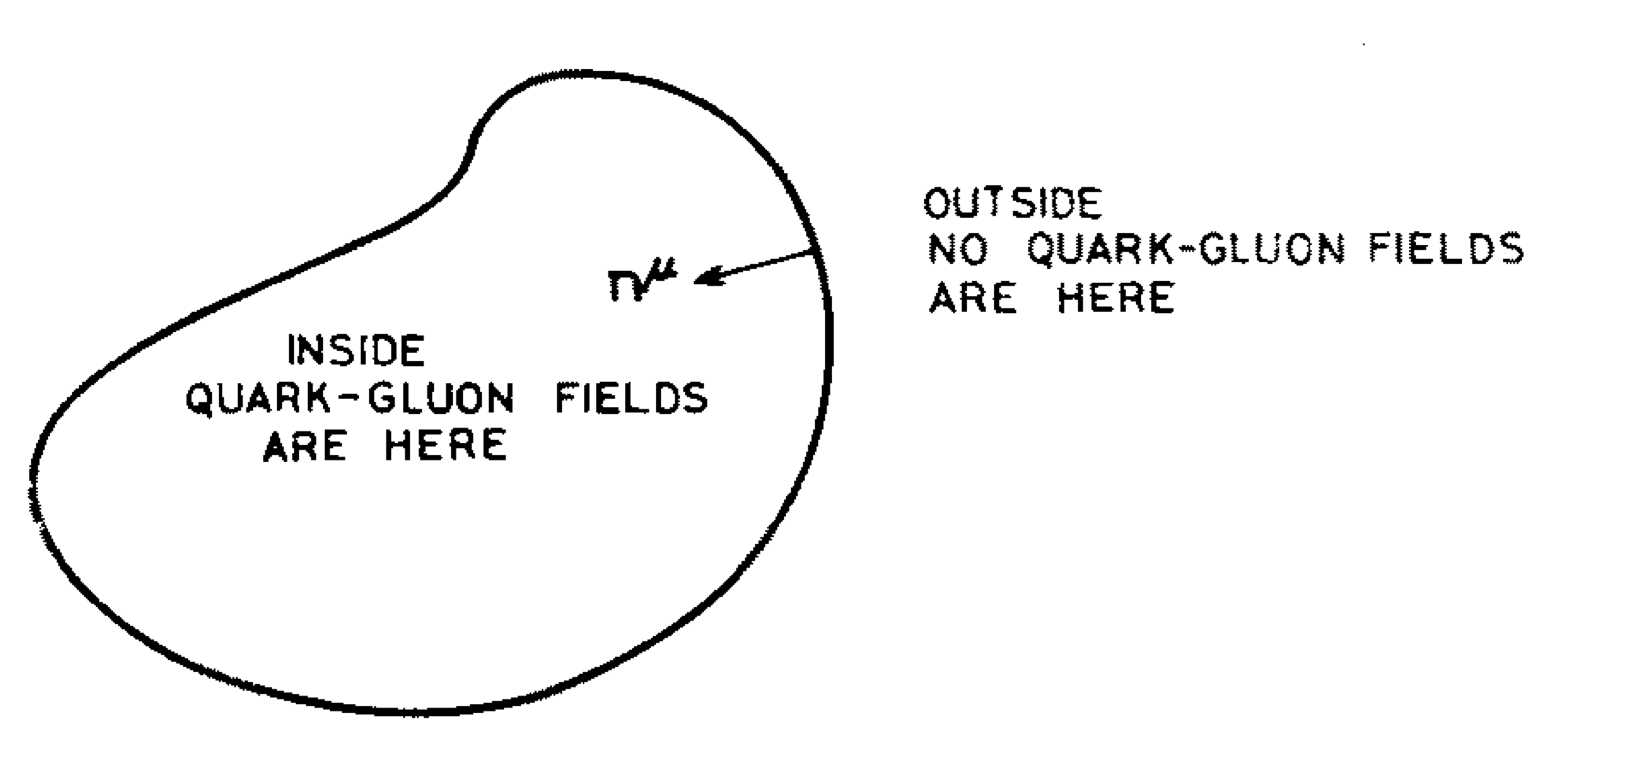
\includegraphics[width=0.5\textwidth]{./Images/Bag model BC.png}
    \caption[Modelo de bolsa con condiciones de frontera]{\emph{Dentro de la bolsa, los quarks están confinados debido a la presión de bolsa que equilibra la presión del vacío exterior.}}
    \label{fig: Bolsa BC}
\end{wrapfigure}

Desde el punto de vista de la \gls{qcd}, el modelo incorpora dos elementos fundamentales:

\begin{enumerate}[i.]
    \item \textbf{Singlete de color:} Las condiciones de frontera del modelo requieren que el estado confinado sea un singlete de color, en consistencia con el principio de confinamiento.
    \item \textbf{Intercambio de gluones:} Aunque el modelo en su forma más simple no incluye campos gluónicos explícitamente, se pueden incorporar como correcciones que contribuyen al espectro de energía de los estados ligados.
\end{enumerate}

A pesar de su simplicidad, el modelo ha mostrado ser efectivo al capturar ciertas características de los hadrones. En esta tesis, extendemos este marco incorporando conceptos de la estadística no extensiva de \gls{tsallis}, con el objetivo de explorar nuevas formas de describir la energía, temperatura y presión internas del protón.

\section{La aproximación de la cavidad esférica}

Una de las aproximaciones más utilizadas en el \gls{bm} es considerar que los quarks se encuentran confinados dentro de una región esférica de radio $R_0$, denominada \emph{cavidad esférica}. Esta simplificación permite resolver las ecuaciones del sistema bajo condiciones bien definidas, preservando los aspectos esenciales del confinamiento.

La dinámica de los quarks en esta configuración esférica se describe mediante una acción efectiva \cite{Chodos_1974}, que incluye los términos correspondientes a la energía cinética, energía de masa, presión de bolsa, y una condición de frontera:

\begin{equation} \label{eq:bag-action}
W = \int \! \mathrm{d}t \left[ \int_V \! \mathrm{d}^3x \left( \frac{i}{2} \bar{\psi} \overleftrightarrow{\partial}_{\mu} \gamma^\mu \psi - \bar{\psi} m \psi - B \right) - \frac{1}{2} \int_S \! \mathrm{d}^2x \, \bar{\psi} \psi \right],
\end{equation}

donde:
\begin{enumerate}
    \item[$\triangleright$] $\psi$ es el \emph{campo de quarks espinorial},
    \item[$\triangleright$] $B$ representa la \emph{presión de bolsa}, que actúa como energía de confinamiento,
    \item[$\triangleright$] $\bar{\psi} \overleftrightarrow{\partial}_{\mu} \gamma^\mu \psi$ es el \emph{término cinético relativista},
    \item[$\triangleright$] $m$ es la \emph{masa de los quarks} (que puede tomarse como nula en el límite relativista),
    \item[$\triangleright$] $V$ es el \emph{volumen de la bolsa} y $S$ su \emph{superficie}.
\end{enumerate}

\paragraph{Ecuaciones de movimiento:}
La ecuación de Dirac dentro de la bolsa se obtiene al variar la acción \eqref{eq:bag-action} con respecto al campo de quarks $\psi$. Esto conduce a:

\begin{equation}\label{eq-deq}
( i \slashed{\partial} - m) \psi= 0 \quad \mathrm{en} \, V,
\end{equation}

donde $\slashed{\partial} = {\partial}_{\mu} {\gamma}^{\mu}$.

\paragraph{Condiciones de frontera:}
Las condiciones de frontera en la superficie $S$ se obtienen al variar la acción \eqref{eq:bag-action} con respecto a la superficie que encierra el volumen $V$. Estas condiciones garantizan que los quarks no puedan escapar de la bolsa y que la presión externa se equilibre con la \emph{presión de bolsa} $B$:

\begin{subequations}\label{eq-bc-deq}
    \begin{empheq}[right=\empheqrbrace \quad \text{sobre} \, S \text{,}]{align}
        i {n}^{\mu} {\gamma}_{\mu} \psi &= \psi \label{eq-bc-deq-a} \\
        \frac{1}{2} {n}_{\mu} {\partial}^{\mu}(\bar{\psi} \psi) &= B \label{eq-bc-deq-b}
    \end{empheq}
\end{subequations}

\subsubsection*{Solución modal de la ecuación de Dirac}

Para resolver \eqref{eq-deq} en coordenadas esféricas, se hace uso de la separación de variables y la expansión en modos normales. La solución general adopta la forma:

\begin{equation} \label{eq:expansion-modos}
\psi(x, t) = \sum_{n\kappa jm} N(\omega_{n\kappa}) a_{n\kappa jm} \, \psi_{n\kappa jm}(x) e^{-i \omega_{n\kappa} t},
\end{equation}

donde:
\begin{enumerate}
    \item[$\triangleright$] $\omega_{n\kappa}$ son las \emph{frecuencias propias} de los modos de oscilación en la bolsa,
    \item[$\triangleright$] $N(\omega_{n\kappa})$ es una \emph{constante de normalización},
    \item[$\triangleright$] $a_{n\kappa jm}$ son \emph{coeficientes de expansión},
    \item[$\triangleright$] $\psi_{n\kappa jm}(x)$ son los \emph{modos normales}.
\end{enumerate}

Cada modo se expresa como un espinor de cuatro componentes en forma:

\begin{equation}
\psi_{n\kappa jm}(r, \theta, \phi) = 
\begin{pmatrix}
f_{n\kappa}(r) \, \Omega_{\kappa jm}(\theta,\phi) \\
i g_{n\kappa}(r) \, \Omega_{-\kappa jm}(\theta,\phi)
\end{pmatrix},
\end{equation}

donde $f_{n\kappa}(r)$ y $g_{n\kappa}(r)$ son funciones radiales obtenidas a partir de las soluciones de Bessel y $\Omega_{\kappa jm}$ son armónicos angulares con espín.

\subsection*{Condición de cuantización y frecuencias permitidas}

La condición de frontera lineal \eqref{eq-bc-deq-a} implica una relación trascendental que fija las frecuencias permitidas dentro de la bolsa \cite{Joseph1981, Chodos_1974, Lagerkvist_2015}. Esta condición se puede expresar como:

\begin{equation} \label{eq:cuantizacion}
\tan(\omega_{n\kappa}) = \frac{\omega_{n\kappa}}{\omega_{n\kappa} + \kappa}.
\end{equation}

O, de forma equivalente:

\begin{equation} \label{eq:bessel-cuanti}
j_0(\omega_{n\kappa}) = - \kappa \, j_1(\omega_{n\kappa}),
\end{equation}

donde:
\[
j_0(x) = \frac{\sin x}{x}, \quad j_1(x) = \frac{\sin x}{x^2} - \frac{\cos x}{x}.
\]

Las primeras raíces de estas ecuaciones determinan los valores discretos de $\omega_{n\kappa}$ que caracterizan los estados cuánticos permitidos. Algunos de los primeros valores son:

\[
\begin{array}{ccc}
\kappa = -1: & \omega_{1,-1} \approx 2.04, & \omega_{2,-1} \approx 5.40 \\
\kappa = +1: & \omega_{1,1} \approx 3.81, & \omega_{2,1} \approx 7.00
\end{array}
\]


\begin{remark}[Sobre los modos espinoriales]
    Para los estados de espín \( j = \frac{1}{2} \), que corresponden a los quarks constituyentes de los hadrones, las soluciones a la ecuación de Dirac bajo las condiciones de frontera \eqref{eq-bc-deq} presentan dos configuraciones relevantes: \( \kappa = \pm 1 \). Estas soluciones modales involucran funciones de Bessel esféricas y espinores angulares, y permiten describir cuantitativamente el comportamiento energético del sistema.

    \paragraph{Soluciones específicas para \( j = \frac{1}{2} \):}
    
    \begin{itemize}
    \item Para \( \kappa = -1 \):
    \begin{equation}
    \psi_{n, -1, \frac{1}{2}, m}(x,t) = \frac{1}{\sqrt{4\pi}} 
    \begin{pmatrix}
    i j_0\left( \frac{\omega_{n,-1} r}{R_0} \right) U_m \\
    - j_1\left( \frac{\omega_{n,-1} r}{R_0} \right) \sigma \cdot \hat{r} \, U_m
    \end{pmatrix}
    e^{-i \omega_{n,-1} t / R_0}
    \end{equation}
    
    \item Para \( \kappa = 1 \):
    \begin{equation}
    \psi_{n, 1, \frac{1}{2}, m}(x,t) = \frac{1}{\sqrt{4\pi}} 
    \begin{pmatrix}
    i j_1\left( \frac{\omega_{n,1} r}{R_0} \right) \sigma \cdot \hat{r} \, U_m \\
    j_0\left( \frac{\omega_{n,1} r}{R_0} \right) U_m
    \end{pmatrix}
    e^{-i \omega_{n,1} t / R_0}
    \end{equation}
    \end{itemize}
    
    donde \( U_m \) es un espinor de Pauli y \( j_\ell(z) \) son las funciones de Bessel esféricas:
    \[
    j_0(x) = \frac{\sin x}{x}, \quad j_1(x) = \frac{\sin x}{x^2} - \frac{\cos x}{x}.
    \]
    
    
    Aunque en este trabajo no se hace uso directo de estas soluciones específicas, su estructura y cuantización son fundamentales para posibles estudios futuros que busquen determinar las masas hadrónicas a partir de la contribución energética de los modos confinados. Esta dirección será brevemente comentada en el capítulo de conclusiones.
\end{remark}

\subsection*{Resultados físicos del modelo}

El modelo permite derivar relaciones relevantes para sistemas hadrónicos. En particular:

\begin{enumerate}[a)]
    \item La energía total de la bolsa es proporcional al volumen promediado:  
    \[
    E = 4B \langle V \rangle.
    \]
    
    \item En el límite termodinámico, el sistema tiene una temperatura característica \( T_0 \sim B^{-1/4} \) (esto se verá en el capítulo \ref{ch-ProtonBagParameters}), independiente de su energía total. Esto implica una densidad de estados de tipo exponencial:
    \[
    \zeta(E) \sim e^{E/T_0}.
    \]
\end{enumerate}

\blankpage